
\documentclass[a4paper,oneside,10pt]{article}
\usepackage[utf8]{inputenc}
\usepackage[T1]{fontenc} 
\usepackage{amsmath,amssymb}
\usepackage{fullpage}
\usepackage{graphicx}
\usepackage{url}
\usepackage{xspace}
\usepackage[french]{babel}
\usepackage{multicol}
\usepackage{geometry}
\usepackage{float}
\geometry{hmargin=2cm,vmargin=1.8cm}
\title{Projet ACVL - Rapport}

\author{DANTIGNY Raynald, DE GEA Jordan, DUCLOT William, RABOURG Simon}

\begin{document}

\maketitle

\tableofcontents


\pagebreak
\section{Analyse}
\subsection{Diagramme de classes d'analyse}
\begin{figure}[H]
\begin{center}
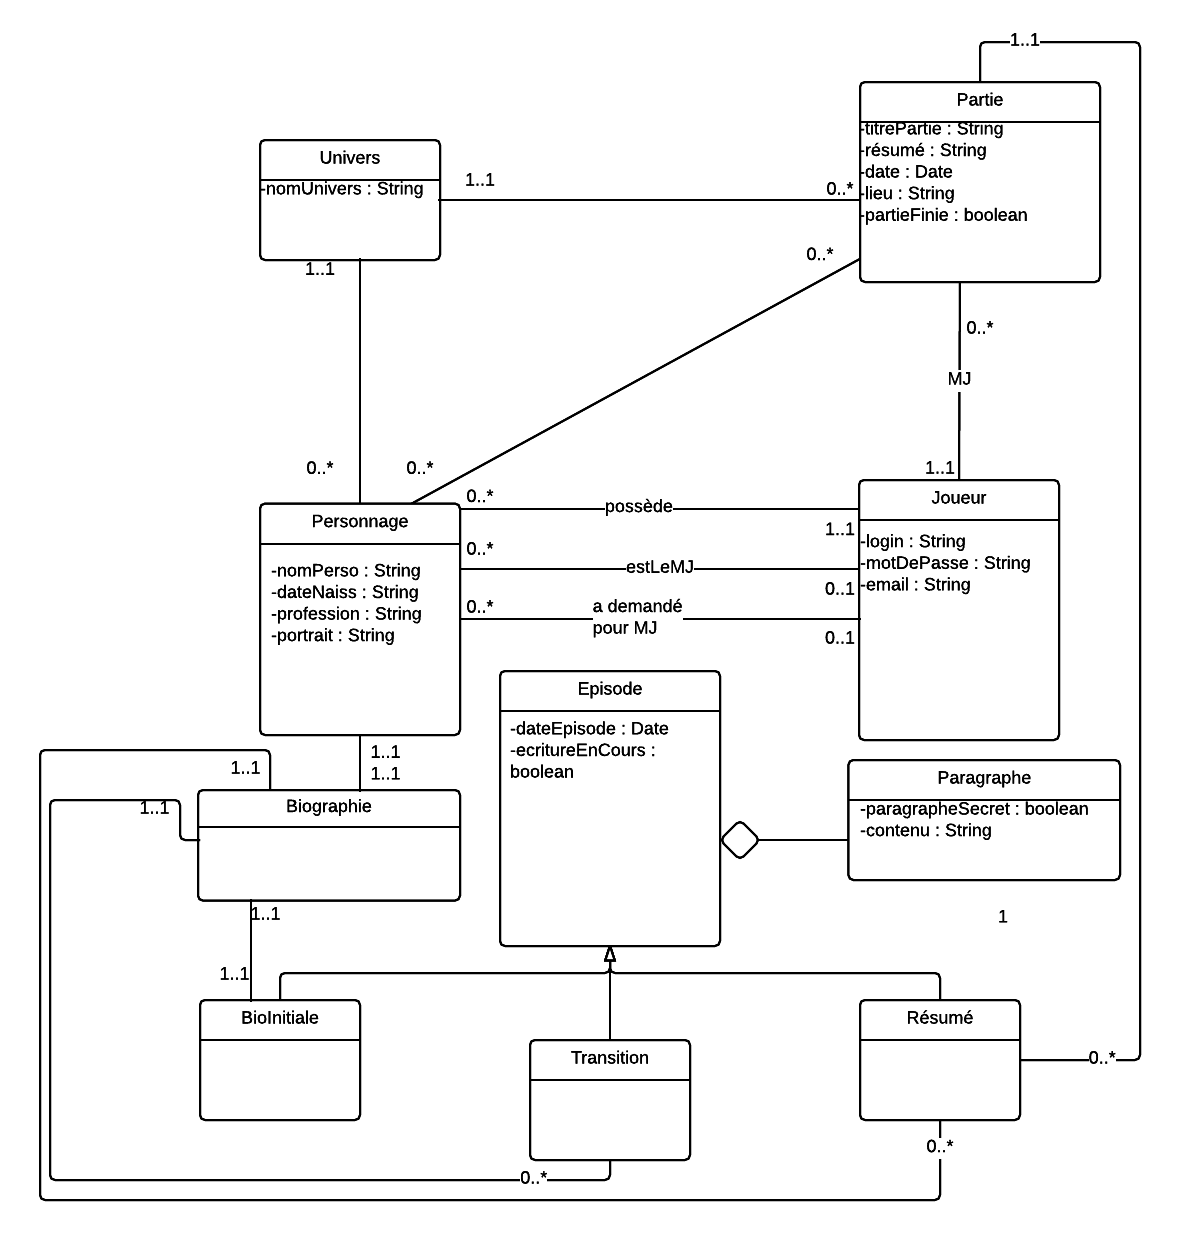
\includegraphics[width=\textwidth]{images/classe/DiagrammeClasse.png} 
	\caption{Diagramme de classes d'analyse}
\end{center}
\end{figure}


\pagebreak
\subsection{Cas d'utilisation}

\begin{figure}[H]
	\begin{center}
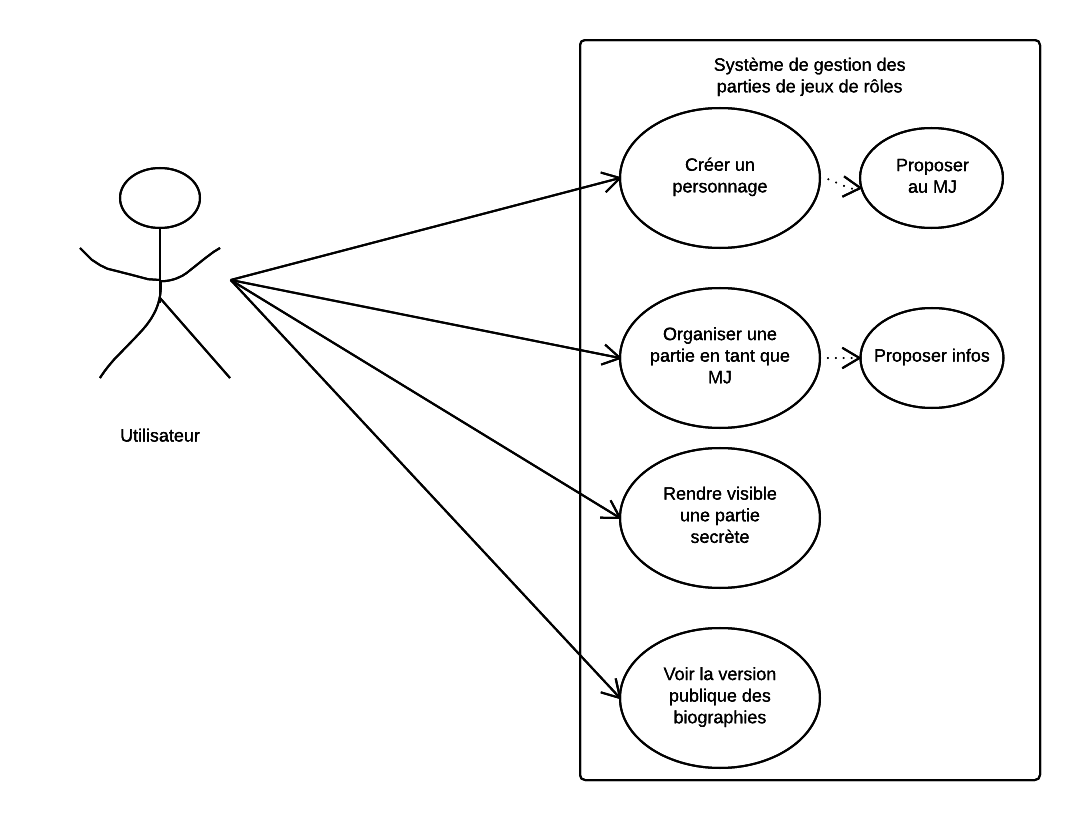
\includegraphics[width=0.6\textwidth]{images/utilisation/UserCU.png} 
	\caption{Cas d'utilisation pour l'utilisateur}
\end{center}
\end{figure}
\begin{figure}[H]
	\begin{center}
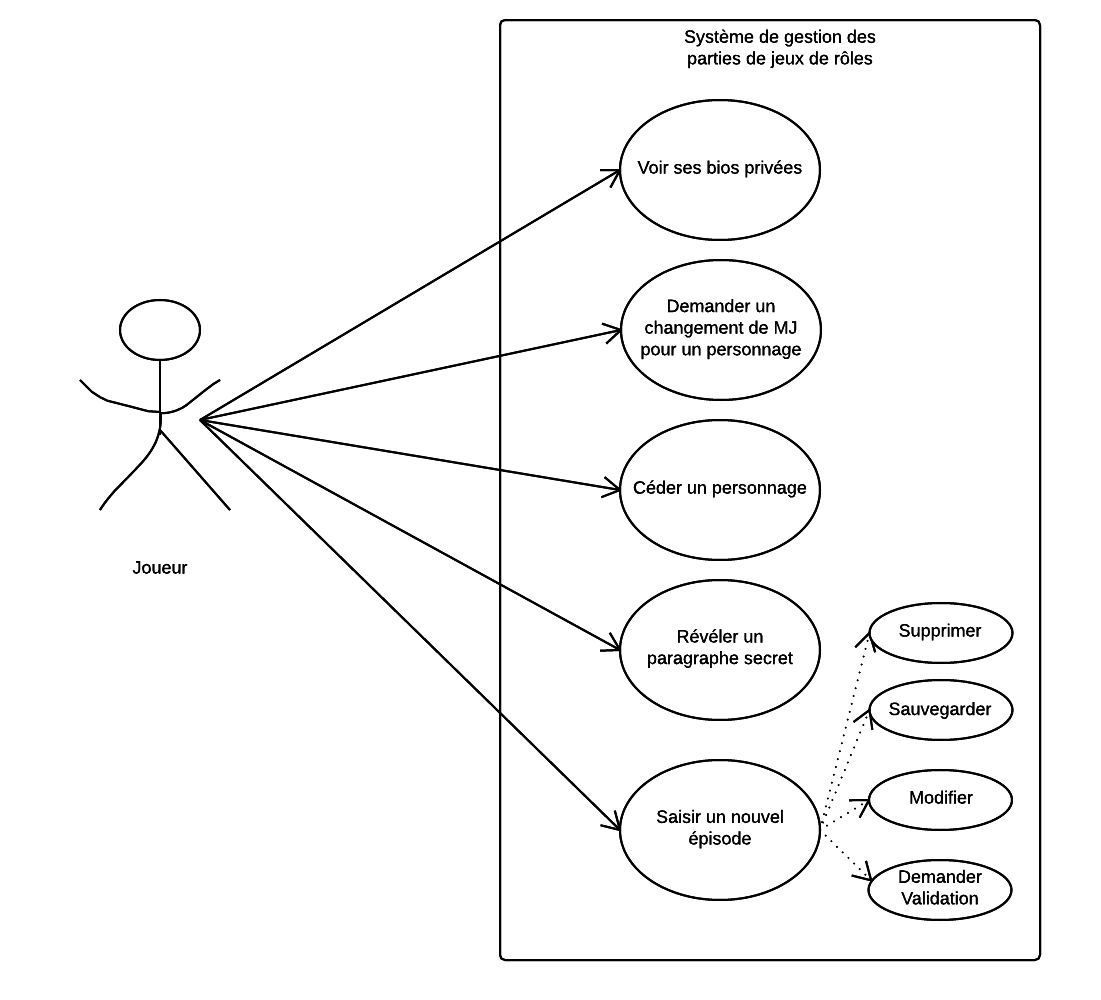
\includegraphics[width=0.49\textwidth]{images/utilisation/JoueurCU.png}
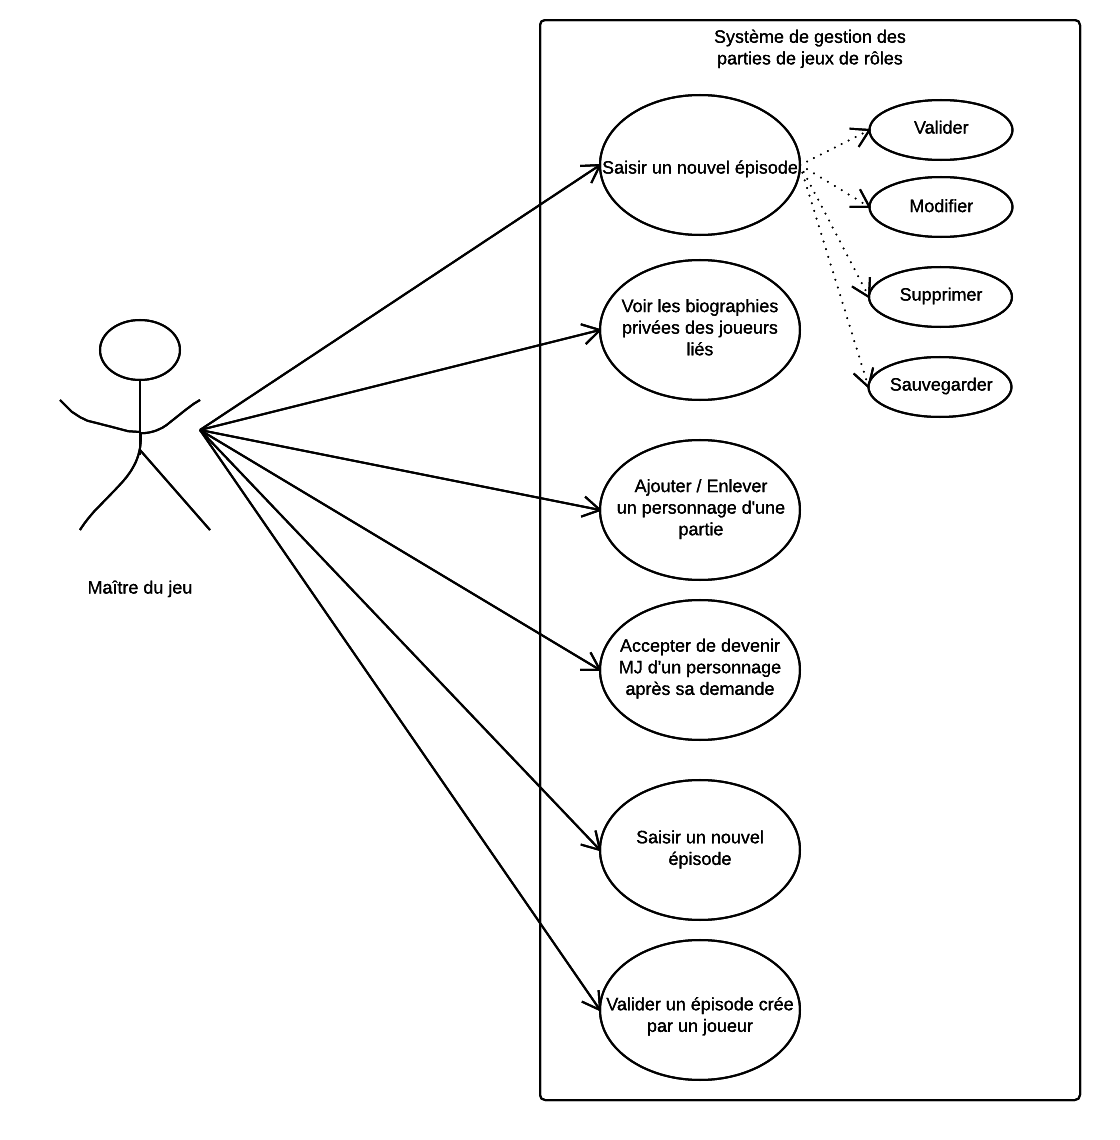
\includegraphics[width=0.49\textwidth]{images/utilisation/MJCU.png}  
	\caption{Cas d'utilisation pour le joueur et le Maitre du Jeu}
\end{center}
\end{figure}

\pagebreak
\subsection{Diagrammes de séquence système}
\begin{figure}[H]
	\begin{center}
		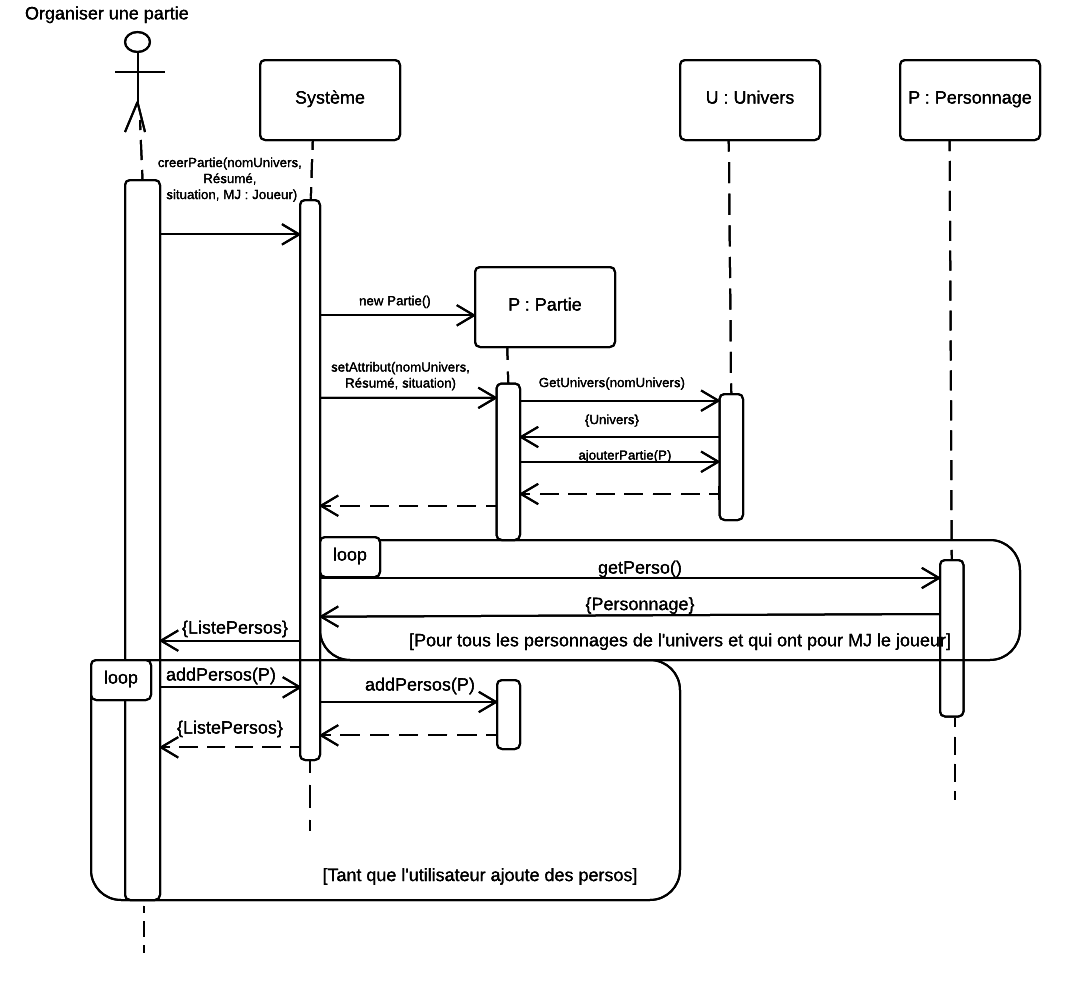
\includegraphics[width=12cm]{images/sequence/DS-OrganiserPartie.png}  
		\caption{Organiser une partie}
	\end{center}
\end{figure}
\begin{figure}[H]
	\begin{center}
		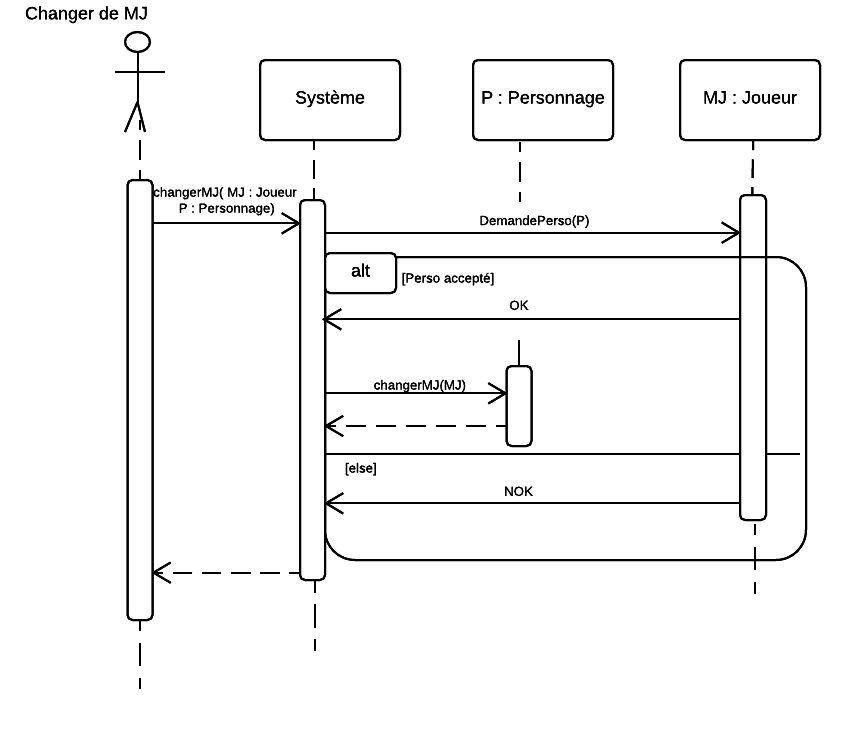
\includegraphics[width=12cm]{images/sequence/DS-ChangerMJ.png}  
		\caption{Changer de maître du jeu pour un personnage}
	\end{center}
\end{figure}
\begin{figure}[H]
	\begin{center}
		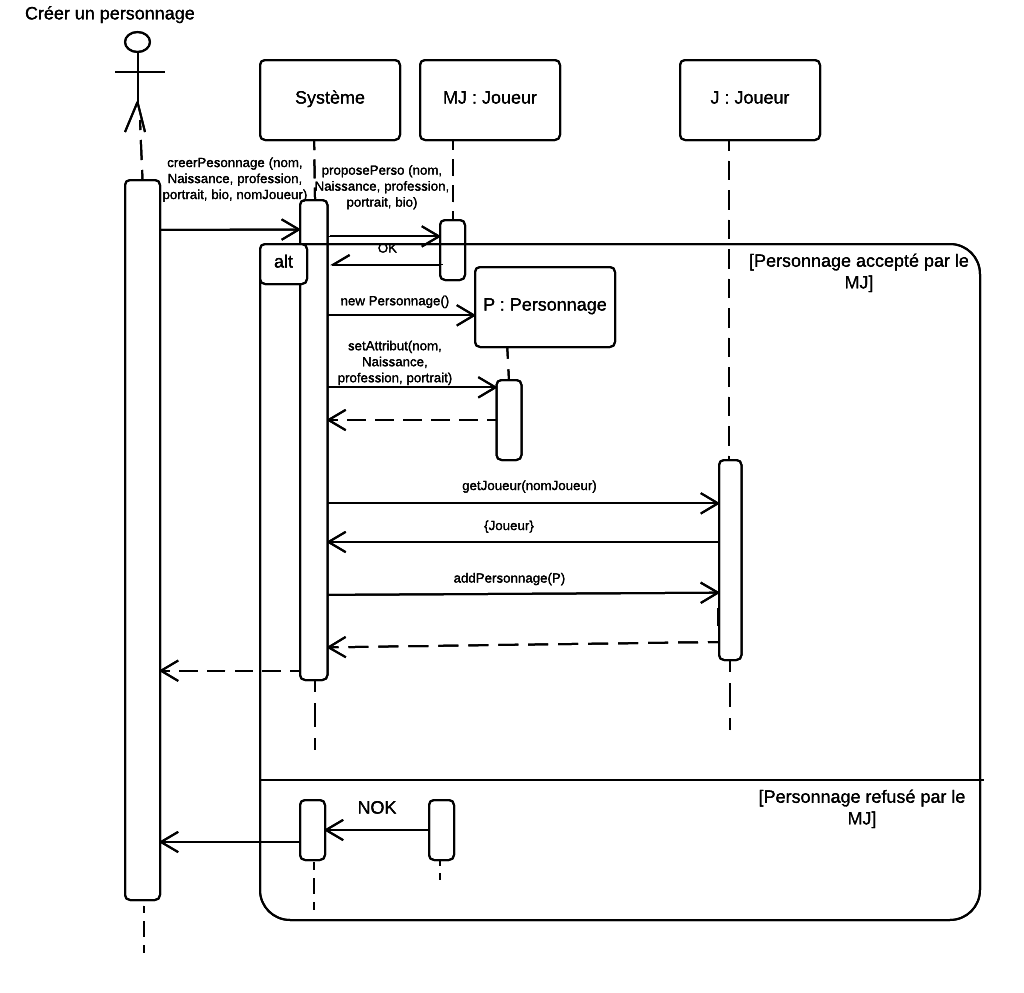
\includegraphics[width=12cm]{images/sequence/DS-CreerPerso.png}  
		\caption{Créer un personnage}
	\end{center}
\end{figure}


\pagebreak

\section{Conception}


\subsection{Diagramme d'architecture MVC}


\subsection{Diagramme de classe logiciel}

\subsection{Diagramme d'Etats-transitions}
\begin{figure}[H]
	\begin{center}
		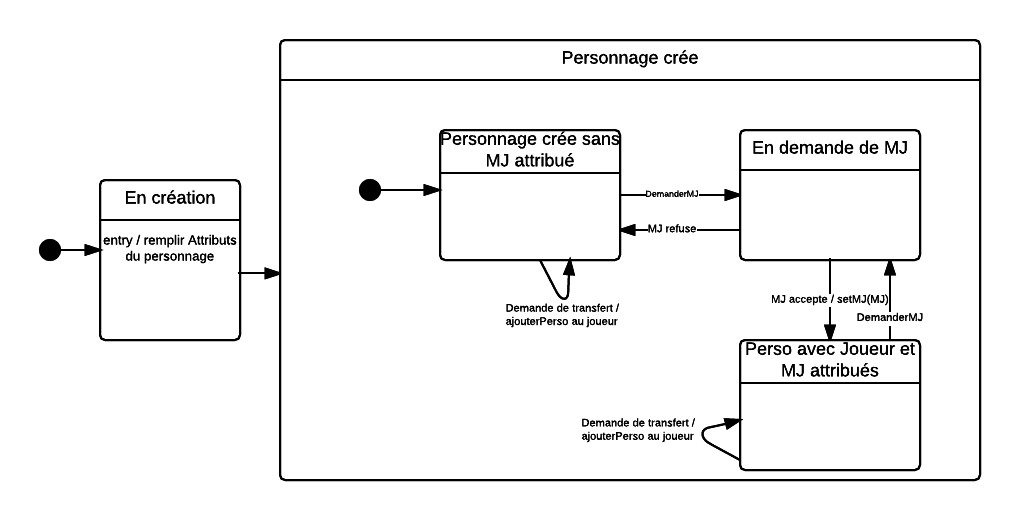
\includegraphics[width=\textwidth]{images/sequence/ET-Personnage.png}  
		\caption{Diagramme d'état/transition pour le changement de MJ et le transfert de personnage}
	\end{center}
\end{figure}

\pagebreak

\section{Manuel Utilisateur}


\pagebreak

\section{Bilan}

%Bilan sur les outils de modélisation utilisés, en particulier les problèmes rencontrés, ainsi que les solutions trouvées. Il vous est demandé dans cette partie de bien préciser les logiciels, en particulier les modeleurs UML que vous avez utilisés.

\subsection{Recherche de modeleurs UML}

Nous avons fait une courte recherche de modeleurs, mais aucun de ceux proposés spécialement en tant que Modeleur ne nous convenait. Nous nous sommes donc dirigé vers un outil que nous connaissons : LucidChart. LucidChart est un outil connecté à GoogleDrive permettant de faire des schémas, d'UML entre autre. 


\subsection{Outil : LucidChart}

Nous avons utilisé LucidChart pour : 
\begin{itemize}
	\item Diagramme de classe d'analyse
	\item Diagramme de séquence système
	\item Cas d'utilisation
\end{itemize}

Difficultés : C'est pratique car c'est personnalisable mais pas forcement adapté pour l'UML. L'utilisation n'est pas simple et intuitive. 

\subsection{IDE : Netbeans}

Nous avons tous utilisé Netbeans pour le développement. L'avantage d'avoir le même IDE est qu'il est plus facile d'aider un collègue lors d'un problème. Etant habitué à cet IDE, nous pouvions développer rapidement. 

\subsection{Tomcat8 / JDBC}

Pour le serveur web, nous avons utilisé Tomcat8 . 
JDBC est la library devant être utilisé pour le projet afin de se connecter à la base Oracle.  

\subsection{Latex : TexMaker}

TexMaker est, selon nous, le meilleur éditeur graphique de contenu \LaTeX. 

\subsection{Versionning : GIT}

Le système de version "de base" pour les projets. Hebergé sur Gitlab.com. 




















\end{document}
